\begin{frame}[allowframebreaks,allowdisplaybreaks]
    \subsubsection{Height}
    \frametitle{B-Tree Properties---Height}
    \begin{columns}
        \begin{column}{\textlecolumn}
            \begin{block}{}
                \begin{itemize}
                    \item Before we can define and prove the height of a B-Tree we need to define some things.
                    \item First, The set of the keys in \(T \in t\left(\alpha, h\right)\) will be defined as \(I\). 
                    \item Now, The \(I_{\text{min}}\) and \(I_{\text{max}}\) of \(T\) can be easily defined by \eqref{btree-nodes-num}:
                \end{itemize}
            \end{block}
            \vspace{-0.35cm}
            \begin{tcolorbox}[boxsep=0mm,left=0mm,right=0mm,top=-2mm,halign=right]
                \[
                    1 + 2\frac{\left(\left(\alpha + 1\right)^{h - 1} - 1\right)}{\alpha} 
                    \leq 
                    N\left(T\right) 
                    \leq 
                    \frac{\left(\left(2\alpha + 1\right)^{h} - 1\right)}{2\alpha}
                \]
            \end{tcolorbox}
        \end{column}
        \begin{column}{\textricolumn}
        \end{column}
    \end{columns}
    \begin{columns}
        \begin{column}{0.5\textwidth}
            \vspace{-0.75cm}
            \begin{block}{}
                \[
                    \begin{aligned}
                        I_{\text{min}} &= 1 + \alpha\left(N_{\text{min}}\left(T\right) - 1\right) \\
                        &= 1 + \alpha\left(\frac{2\left(\alpha + 1\right)^{h - 1} - 2}{\alpha}\right) \\
                        &= 2\left(\alpha + 1\right)^{h - 1} - 1
                    \end{aligned}
                \]
            \end{block}
        \end{column}
        \begin{column}{0.5\textwidth}
            \begin{figure}
                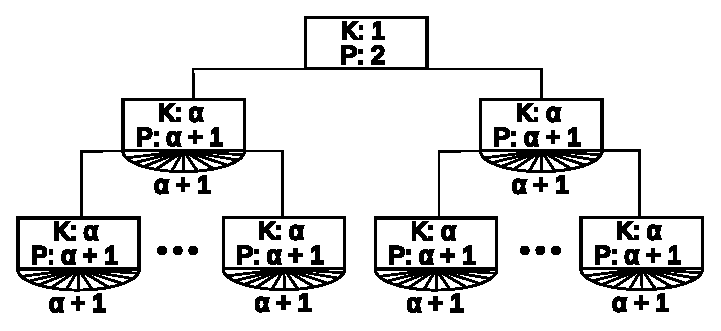
\includegraphics[width=0.95\linewidth,keepaspectratio]{resources/made/generic_min_btree.eps}
                \caption[]{B-Tree w/ the least number of nodes}
            \end{figure}
        \end{column}
    \end{columns}

    \framebreak

    \begin{columns}
        \begin{column}{0.5\textwidth}
            \begin{block}{}
                \vspace{-0.75cm}
                \[
                    \begin{aligned}
                        I_{\text{max}} &= 2\alpha\left(N_{\text{max}}\left(T\right)\right) \\
                        &= 2\alpha \left(\frac{\left(2\alpha + 1\right)^h - 1}{2\alpha}\right) \\
                        &= \left(2\alpha + 1\right)^h - 1
                    \end{aligned}
                \]
            \end{block}
        \end{column}
        \begin{column}{0.5\textwidth}
            \begin{figure}
                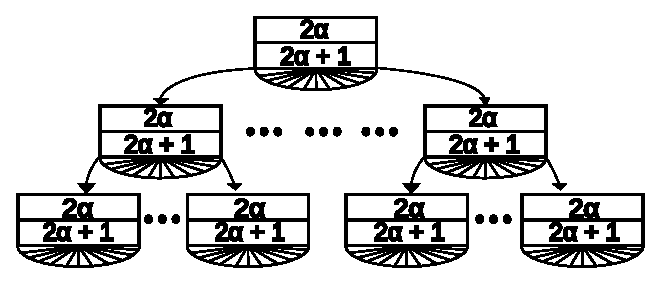
\includegraphics[width=0.95\linewidth,keepaspectratio]{resources/made/generic_max_btree.eps}
                \caption[]{B-Tree w/ the most number of nodes}
            \end{figure}
        \end{column}
    \end{columns}
    \begin{itemize}
        \item Now, we can solve for \(h\) with each bound of \(I\) and define an bound of h with them.
    \end{itemize}
    \begin{columns}
        \begin{column}{0.5\textwidth}
            \begin{block}{}
                \[
                    \begin{aligned}
                        I_{\text{min}} &= 2\left(\alpha + 1\right)^{h - 1} - 1 \\
                        \frac{I_{\text{min} + 1}}{2} &= \left(\alpha + 1\right)^{h - 1} \\
                        \log_{\alpha + 1}\left(\frac{I_{\text{min}} + 1}{2} + 1\right) &= h_{\text{min}}
                    \end{aligned}
                \]
            \end{block}
        \end{column}
        \begin{column}{0.5\textwidth}
            \[
                \begin{aligned}
                    I_{\text{max}} &= \left(2\alpha + 1\right)^h - 1 \\
                    I_{\text{max}} + 1 &= \left(2\alpha + 1\right)^h \\
                    \log_{2\alpha + 1} \left(I_{\text{max}} + 1\right) = h_{\text{max}}
                \end{aligned}
            \]
        \end{column}
    \end{columns}

    \framebreak

    \begin{columns}
        \begin{column}{\textlecolumn}
            \begin{block}{}
                \begin{itemize}
                    \item Since, \(2\alpha + 1 > \alpha + 1\), then \(log_{2\alpha + 1} x \leq log_{\alpha + 1}x\), both in \(\left[1, \infty\right)\).
                    \item Or also, if we have more nodes in a B-Tree, the height of the Tree will be less than if we have less nodes in the B-Tree.
                    \item Hence, for \(I \geq 1\), we will have the bounds for \(h\):
                \end{itemize}
                \[
                    \log_{2\alpha + 1}\left(I + 1\right)
                    \leq
                    h
                    \leq
                    \log_{\alpha + 1}\left(\frac{I + 1}{2} + 1\right)
                \]
                \begin{itemize}
                    \item And if, \(I = 0\) then, \(h = 0\).
                \end{itemize}
            \end{block}
        \end{column}
        \begin{column}{\textricolumn}
        \end{column}
    \end{columns}
\end{frame}
